% SPDX-License-Identifier: BUSL-1.1
% Copyright (c) 2025-2026 Lucas Ricardo Mella Chillemi
%
% PAMPAr-Coder V3: Brain-Inspired 2D Stream Architecture with Mixed Selectivity
% Prepared for arXiv submission (cs.CL / cs.LG)
%
\documentclass[11pt,a4paper]{article}

% ============================================================================
% PACKAGES
% ============================================================================
\usepackage[utf8]{inputenc}
\usepackage[T1]{fontenc}
\usepackage{amsmath,amssymb,amsfonts}
\usepackage{graphicx}
\usepackage{booktabs}
\usepackage{hyperref}
\usepackage{cleveref}
\usepackage{algorithm}
\usepackage{algorithmic}
\usepackage{tikz}
\usetikzlibrary{shapes,arrows,positioning,fit,backgrounds,calc}
\usepackage[margin=1in]{geometry}
\usepackage{natbib}
\usepackage{xcolor}
\usepackage{multirow}

% Placeholder macro for pending ablation values
\newcommand{\placeholder}[1]{\textcolor{gray}{\textit{#1}}}

% ============================================================================
% METADATA
% ============================================================================
\title{PAMPAr-Coder V3: A Brain-Inspired 2D Stream Architecture\\
with Mixed Selectivity for Efficient Code Generation}

\author{
Lucas Ricardo Mella Chillemi\\
Independent Researcher\\
Buenos Aires, Argentina\\
\texttt{lucas.mella@outlook.com}
}

\date{April 2026\\[1em]
\small DOI: \href{https://doi.org/10.57967/hf/8329}{10.57967/hf/8329}\\
\small Model: \href{https://huggingface.co/lucas-mella/PAMPAr-Coder}{lucas-mella/PAMPAr-Coder}
}

% ============================================================================
% DOCUMENT
% ============================================================================
\begin{document}

\maketitle

% ============================================================================
% ABSTRACT
% ============================================================================
\begin{abstract}
We present PAMPAr-Coder V3, a compact code generation language model of 62.6M
parameters designed for consumer GPUs with as little as 4GB VRAM.  The
architecture extends the PAMPAr lineage of brain-inspired models with two novel
contributions: (1) a \textit{2D Stream} organization that arranges computation
as four specialized cortical streams (Syntax, Semantics, Logic, Structural)
across five depth levels, connected by bidirectional lateral gates analogous to
white-matter fiber tracts; and (2) \textit{Mixed Selectivity} via Feature-wise
Linear Modulation (FiLM), where a single shared Feed-Forward Network is
dynamically re-read by context-dependent $\gamma/\beta$ modulators derived from
a 63-dimensional context vector — reducing FFN parameters by $\sim$72\% per
level compared to four independent networks.  A lightweight Tálamo re-routing
module at each depth level allows token-territory assignments to drift as
context evolves, and a Zone-of-Proximal-Development (ZPD) curriculum
(\textit{MotorCuriosidad}) adapts training difficulty in real time across 161
topic categories and 3.2M lines of code data.  After 55,000 training steps on
a GTX~1650 (4.3~GB VRAM), V3 reaches a cross-entropy loss of $\sim$1.38 on the
validation set and saturates 29 of 40 curriculum topics.  We argue that
horizontal stream specialization combined with vertical depth, lateral
communication, and context-modulated parameter sharing constitutes a promising
direction for efficient, interpretable code models.
\end{abstract}

\textbf{Keywords:} code generation, brain-inspired architecture, mixed
selectivity, FiLM modulation, grouped-query attention, curriculum learning,
parameter efficiency, ZPD

% ============================================================================
% 1. INTRODUCTION
% ============================================================================
\section{Introduction}
\label{sec:introduction}

Large language models (LLMs) for code—CodeLlama \citep{roziere2023code},
StarCoder2 \citep{lozhkov2024starcoder2}, DeepSeek-Coder
\citep{guo2024deepseek}—achieve state-of-the-art results at the cost of
billions of parameters and tens of gigabytes of GPU memory, placing them out of
reach for local, privacy-preserving, or resource-constrained deployments.
Distillation to smaller models (1–3B) partially alleviates this, but even
1.3B-parameter models require careful quantization to fit on a consumer 4GB
GPU and still represent a $\sim$20$\times$ larger parameter budget than
what we demonstrate here.

At the same time, biological neural systems process language (and implicitly,
structured logical sequences) with remarkable efficiency through functional
specialization and modulatory dynamics: cortical areas maintain distinct
computational identities while sharing representational substrates via
inter-areal projections \citep{felleman1991distributed}, and individual neurons
exhibit \emph{mixed selectivity} — responding to conjunctions of context,
task, and content that would otherwise require an exponential number of
specialized units \citep{rigotti2013importance}.

PAMPAr-Coder V3 is motivated by these two observations.  Its contributions are:

\begin{enumerate}
    \item \textbf{2D Stream Architecture}: computation organized as a
    $N_\text{streams} \times N_\text{levels}$ grid, where each stream
    specializes in a syntactic/semantic/logical/structural role across
    five depth levels, with lateral gates at each level enabling controlled
    inter-stream information exchange (\cref{sec:architecture}).

    \item \textbf{Mixed Selectivity via FiLM}: a single shared FFN per level
    modulated by four stream-specialized $(\gamma, \beta)$ pairs derived from
    a 63-dimensional context descriptor — zone activations, territorial
    activations, depth, confidence, and stream identity (\cref{sec:mixed}).

    \item \textbf{Adaptive Tálamo Re-routing}: a lightweight per-level
    module that updates token-territory allocations as stream states evolve,
    allowing routing to ``drift'' from initial LLAVES assignments
    (\cref{sec:talamo}).

    \item \textbf{ZPD Curriculum (MotorCuriosidad)}: a curiosity-driven
    scheduler that selects training batches from topics at the boundary of
    competence, enabling stable learning across 161 heterogeneous topic
    categories without manual weighting (\cref{sec:curriculum}).
\end{enumerate}

The result is a 62.6M-parameter model trainable end-to-end on a 4GB consumer
GPU in a single day, reaching competitive code generation behavior while
remaining interpretable at the routing level.

% ============================================================================
% 2. RELATED WORK
% ============================================================================
\section{Related Work}
\label{sec:related}

\subsection{Compact Code Language Models}

PolyCoder \citep{xu2022systematic} demonstrated that small models ($\leq$2.7B)
trained exclusively on code can outperform general-purpose LLMs on specific
languages.  CodeT5+ \citep{wang2023codet5plus} introduced encoder-decoder
architectures for code with strong results at 220M parameters.  Our model
occupies a more extreme point in this space at 62.6M parameters, aimed at
deployments where even 220M is expensive.

\subsection{Parameter-Efficient Architectures}

Grouped-Query Attention (GQA) \citep{ainslie2023gqa} reduces key-value cache
memory by sharing KV heads across query groups; we use a 4:1 ratio (8Q:2KV)
that cuts KV parameters significantly.  Mixture-of-Experts (MoE)
\citep{shazeer2017outrageously} achieves parameter efficiency through sparse
activation; our stream architecture achieves a related specialization through
hard territorial assignments rather than learned sparse routing.  ALBERT
\citep{lan2019albert} uses cross-layer parameter sharing; our Mixed
Selectivity approach generalizes this: instead of sharing \emph{the same}
FFN across layers, we share one FFN per level across streams and modulate it
contextually.

\subsection{Feature-wise Linear Modulation}

FiLM \citep{perez2018film} conditions a neural network's internal features
via element-wise affine transformations $\hat{h} = \gamma \odot h + \beta$
where $\gamma, \beta$ are produced by an auxiliary network.  It has been
applied to visual question answering, game playing, and multi-task learning.
To our knowledge, this is the first application of FiLM-style modulation to
a language model's FFN sub-layers for stream specialization.

\subsection{Mixed Selectivity in Neuroscience and AI}

\citet{rigotti2013importance} showed that mixed selectivity — neurons
responding to combinations of stimuli rather than single features — is
critical for flexible, generalizable behavior in prefrontal cortex.
\citet{elhage2022toy} (Anthropic) demonstrated that transformers can
represent more concepts than dimensions through superposition, effectively
implementing mixed selectivity.  Our ContextModulator operationalizes this:
the shared FFN encodes a ``dictionary'' of code transformations, and each
stream selects and scales relevant entries through $\gamma/\beta$ modulation.

\subsection{Curriculum and Adaptive Learning}

Self-paced learning \citep{kumar2010self} orders training examples by
difficulty.  Power-law curricula \citep{bengio2009curriculum} smooth the
transition from easy to hard.  Our ZPD-based MotorCuriosidad is closest to
competence-based progression \citep{florensa2017reverse}: a topic advances
only when the model reaches a dominance threshold, preventing overfitting on
mastered topics and catastrophic forgetting of partially learned ones.

\subsection{PAMPAr Lineage}

PAMPAr-o1 v9 \citep{mella2026pampar} introduced territorial computing for
general language modeling with a hybrid LLAVES-attention routing system,
achieving $\sim$45 perplexity on WikiText-103 with 14M parameters.
PAMPAr-Coder V3 extends this lineage to code, scaling parameters $\times$4.5,
introducing the FiLM modulatory pathway, replacing flat territorial blocks with
the 2D stream-level grid, and targeting a specialized 48K code-biased
vocabulary.

% ============================================================================
% 3. ARCHITECTURE
% ============================================================================
\section{Architecture Overview}
\label{sec:architecture}

PAMPAr-Coder V3 consists of five components:
(i) a SentencePiece embedding layer (48K vocab, dim=640),
(ii) a global Tálamo router producing initial territory assignments,
(iii) a $4 \times 5$ stream-level grid of NivelProfundo blocks,
(iv) per-level TalamoNivel re-routing modules,
(v) a tied output projection.

\Cref{fig:architecture} illustrates the overall structure.

\begin{figure}[t]
\centering
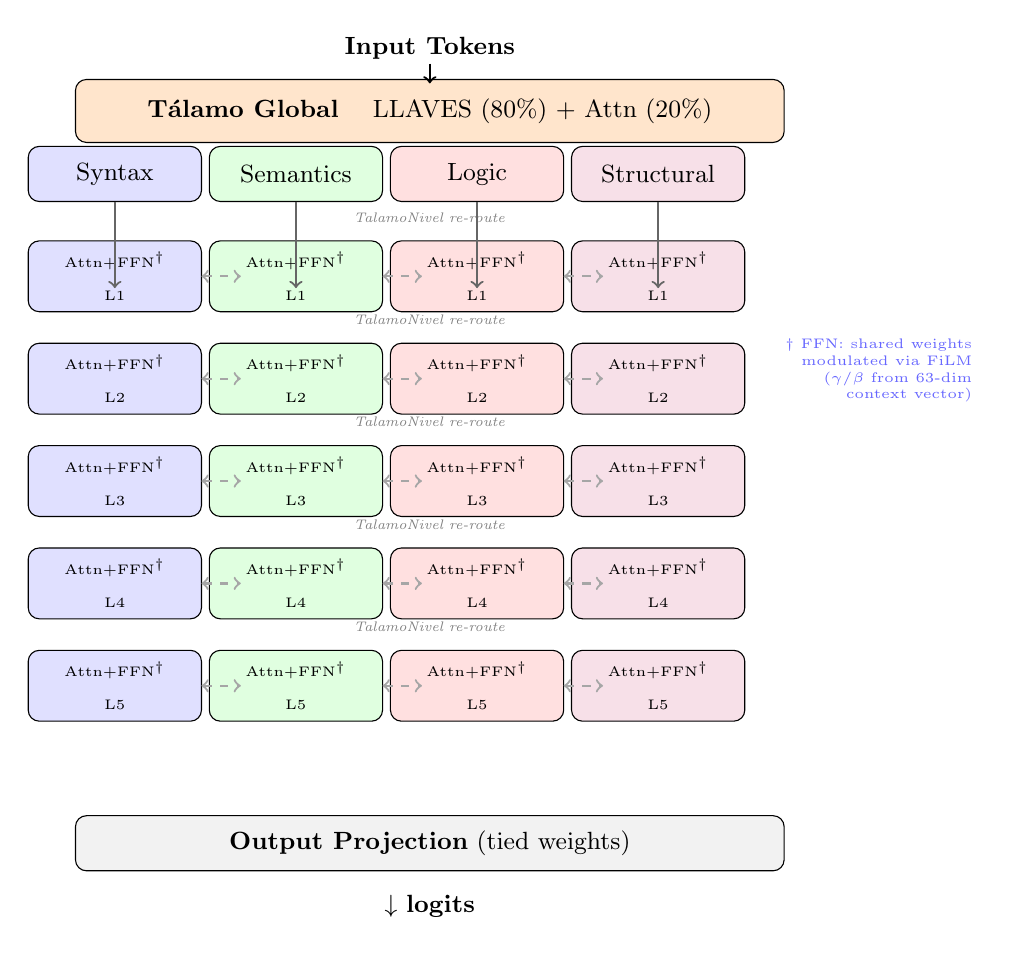
\begin{tikzpicture}[
    stream/.style={draw, rounded corners, minimum width=2.2cm,
                   minimum height=1.0cm, align=center, font=\small},
    level_label/.style={font=\footnotesize\itshape, align=center},
    talamo/.style={draw, rounded corners, fill=orange!20,
                   minimum width=9cm, minimum height=0.8cm,
                   align=center, font=\small},
    lateral/.style={<->, dashed, thick, gray!70},
    down/.style={->, thick, black!60},
    syn/.style={fill=blue!12},
    sem/.style={fill=green!12},
    log/.style={fill=red!12},
    str/.style={fill=purple!12},
]

% Global Talamo
\node[talamo] (talamo) at (4.5, 9.8)
    {\textbf{Tálamo Global} \quad LLAVES (80\%) + Attn (20\%)};

% Column labels
\foreach \name/\col/\style in {
    Syntax/0/syn, Semantics/1/sem, Logic/2/log, Structural/3/str}
{
    \node[stream, \style, minimum height=0.7cm]
        at (\col*2.3+0.5, 9.0) {\small\name};
}

% Grid of NivelProfundo blocks
\foreach \lvl in {1,...,5} {
    \pgfmathsetmacro\y{9.0 - \lvl*1.3}
    % TalamoNivel re-routing (between levels)
    \node[font=\tiny, gray] at (4.5, \y+0.75)
        {\textit{TalamoNivel re-route}};
    \foreach \col/\style in {0/syn, 1/sem, 2/log, 3/str} {
        \node[stream, \style, minimum height=0.9cm]
            at (\col*2.3+0.5, \y)
            {\tiny Attn+FFN$^\dagger$\\[1pt]\tiny L\lvl};
    }
    % Lateral gates
    \foreach \a/\b in {0/1, 1/2, 2/3} {
        \pgfmathsetmacro\xa{\a*2.3+1.6}
        \pgfmathsetmacro\xb{\b*2.3-0.2}
        \draw[lateral] (\xa, \y) -- (\xb, \y);
    }
}

% Arrows from Talamo to level 1
\foreach \col in {0,...,3} {
    \draw[down] (\col*2.3+0.5, 8.65) -- (\col*2.3+0.5, 7.5+0.05);
}

% Output
\node[talamo, fill=gray!10, minimum width=9cm, minimum height=0.7cm]
    at (4.5, 0.5) {\textbf{Output Projection} (tied weights)};

% Vertical flow
\node at (4.5, -0.3) {\small$\downarrow$ \textbf{logits}};
\node at (4.5, 10.6) {\small\textbf{Input Tokens}};
\draw[->, thick] (4.5, 10.4) -- (4.5, 10.15);

% FiLM annotation
\node[font=\tiny, align=right, text=blue!60] at (10.2, 6.5)
    {$\dagger$ FFN: shared weights\\modulated via FiLM\\($\gamma/\beta$ from 63-dim\\context vector)};

\end{tikzpicture}
\caption{PAMPAr-Coder V3 architecture.  Four cortical streams (Syntax,
Semantics, Logic, Structural) each process tokens through 5 depth levels.
At each level, lateral gates (dashed arrows) enable inter-stream communication.
A global Tálamo produces initial territory assignments; lightweight
TalamoNivel modules re-route at each depth.  ${}^\dagger$The FFN weights
are \emph{shared} across the 4 streams at each level and modulated by
stream-specific $(\gamma, \beta)$ pairs derived from a 63-dim context vector
(Mixed Selectivity / FiLM).}
\label{fig:architecture}
\end{figure}

\paragraph{Configuration summary.}

\begin{table}[h]
\centering
\small
\begin{tabular}{ll}
\toprule
\textbf{Hyperparameter} & \textbf{Value} \\
\midrule
Vocabulary size        & 48,000 (PAMPAr-48k SentencePiece BPE) \\
Embedding dimension    & 640 \\
Number of streams      & 4 (Syntax, Semantics, Logic, Structural) \\
Number of levels       & 5 \\
Attention heads (Q/KV) & 8Q / 2KV (GQA, ratio 4:1) \\
Head dimension         & 80 \\
FFN hidden dimension   & $\lfloor 2/3 \times 640 \times 4.0 \rfloor \approx 1707$ \\
Lateral bottleneck     & 128 \\
Modulator bottleneck   & 128 \\
Max sequence length    & 4096 tokens \\
Dropout                & 0.1 \\
Brodmann zones (LLAVES)& 52 \\
Total parameters       & 62.6M \\
\bottomrule
\end{tabular}
\caption{Model configuration for PAMPAr-Coder V3.}
\label{tab:config}
\end{table}

% ============================================================================
% 4. TÁLAMO AND LLAVES ROUTING
% ============================================================================
\section{Tálamo and LLAVES Routing}
\label{sec:talamo}

\subsection{Global Tálamo}

The global Tálamo maps input tokens to territorial activations using a hybrid
rule-learned system.  Each token is first classified into one of 52
\emph{Brodmann zones} — code-specific functional categories inspired by the
Brodmann cortical map — using the LLAVES (``keys'') rule set.

LLAVES for code identifies:
\begin{itemize}\setlength\itemsep{2pt}
    \item \textbf{B01--B10}: Keywords (control flow, definitions, imports)
    \item \textbf{B11--B20}: Data types (int, float, str, list, dict, ...)
    \item \textbf{B21--B30}: Operators and punctuation
    \item \textbf{B31--B40}: Identifiers and names
    \item \textbf{B41--B50}: String and comment content
    \item \textbf{B51--B52}: Numeric literals, whitespace/indent
\end{itemize}

Zone activations $z \in [0,1]^{52}$ are then aggregated into 4 territorial
activations:

\begin{equation}
    a_t = \sigma\!\left(\sum_{i \in \mathcal{Z}_t} z_i\right), \quad
    t \in \{\text{Syn}, \text{Sem}, \text{Log}, \text{Str}\}
    \label{eq:territory_agg}
\end{equation}

where $\mathcal{Z}_t$ is the subset of zones assigned to territory $t$.  The
final routing blends LLAVES with a lightweight learned attention projection:

\begin{equation}
    \tilde{a}_t = \eta \cdot a_t^\text{LLAVES}
              + (1-\eta) \cdot \sigma(W_t x)
    \label{eq:hybrid_routing}
\end{equation}

with $\eta = 0.8$ (80\% rule-based, 20\% learned), providing interpretable
routing while allowing adaptation to corpus-specific token patterns.

\subsection{TalamoNivel Re-routing}

A static initial assignment may be suboptimal deeper in the network.
Consider the token \texttt{for}: at level 1 it is correctly classified as a
control-flow keyword (Syntax stream), but at level 3, within a complex
list comprehension, the semantic interpretation may shift substantially toward
the Semantics stream.

TalamoNivel re-routing addresses this with a lightweight per-level module:

\begin{equation}
    a_t^{(\ell)} = \alpha \cdot a_t^{(\ell-1)}
                 + (1-\alpha) \cdot \sigma(W_\ell x^{(\ell)})
    \label{eq:talamo_nivel}
\end{equation}

where $x^{(\ell)}$ is the mean-pooled stream state at level $\ell$,
$\alpha = 0.7$ controls inertia, and $W_\ell \in \mathbb{R}^{D \times 52}$
is a single linear projection (33K parameters).  This design ensures smooth,
non-oscillating drift rather than abrupt routing changes.

% ============================================================================
% 5. MIXED SELECTIVITY (FiLM FFN)
% ============================================================================
\section{Mixed Selectivity via FiLM Modulation}
\label{sec:mixed}

\subsection{Motivation}

A standard 4-stream, 5-level architecture would instantiate
$4 \times 5 = 20$ independent FFN modules.  With hidden dimension 1707,
each SwiGLU FFN has $\sim$2.2M parameters, totaling $\sim$44M for FFNs alone
— 70\% of the model budget.  Mixed Selectivity offers an alternative inspired
by the neuroscientific finding \citep{rigotti2013importance} that prefrontal
neurons achieve behaviorally flexible representations not by specializing to
single stimuli, but by responding to \emph{conjunctions} of context and
content.

\subsection{Architecture}

At each level $\ell$, instead of four independent FFNs, we use:

\begin{itemize}
    \item One \textbf{SharedFFN} (SwiGLU, $\sim$2.2M params) that encodes
    domain knowledge shared across all streams at this level.
    \item Four \textbf{ContextModulators}, one per stream, each generating
    a pair $(\gamma_s, \beta_s) \in \mathbb{R}^{D}$ from a
    63-dimensional context vector $c_s$.
\end{itemize}

The modulated output for stream $s$ at position $i$ is:

\begin{equation}
    \hat{h}_{s,i} = \gamma_s(c_{s,i}) \odot \text{FFN}(h_{s,i})
                  + \beta_s(c_{s,i})
    \label{eq:film}
\end{equation}

where $\odot$ is element-wise multiplication and
$(\gamma_s, \beta_s) = W_2^\top \text{SiLU}(W_1^\top c_{s,i})$
with $W_1 \in \mathbb{R}^{63 \times 128}$, $W_2 \in \mathbb{R}^{128 \times 2D}$.

\subsection{Context Vector Composition}

The 63-dimensional context vector $c_s$ is composed of:

\begin{equation}
    c_s = \left[
        z \in \mathbb{R}^{52},\;
        a \in \mathbb{R}^{4},\;
        \frac{\ell}{L} \in \mathbb{R},\;
        \text{conf} \in \mathbb{R},\;
        L \in \mathbb{R},\;
        e_s \in \mathbb{R}^{4}
    \right]
    \label{eq:context_vector}
\end{equation}

where $z$ are LLAVES zone activations, $a$ are territorial activations,
$\ell/L$ is normalized depth, $\text{conf}$ is the model's current
confidence estimate, $L$ is the total number of levels (for
depth-invariant normalization), and $e_s$ is the one-hot stream identity.
This contextual richness enables the SharedFFN to be read as a different
``functional program'' depending on where, what, and how confident the
model is at each step.

\subsection{Parameter Analysis}

\begin{table}[h]
\centering
\small
\begin{tabular}{lccc}
\toprule
\textbf{Design} & \textbf{FFN params/level} & \textbf{Total (5 levels)} & \textbf{Saving}\\
\midrule
Independent FFNs (4$\times$) & 8.8M & 44.0M & --- \\
Shared + 4 Modulators        & 2.4M & 12.0M & 73\% \\
\midrule
\textbf{V3 (Mixed Selectivity)} & \textbf{2.4M} & \textbf{12.0M} & \textbf{$-$32M} \\
\bottomrule
\end{tabular}
\caption{FFN parameter budget comparison.  Mixed Selectivity saves $\sim$32M
parameters while maintaining per-stream functional specialization through
contextual modulation.}
\label{tab:ffn_budget}
\end{table}

% ============================================================================
% 6. LATERAL GATES
% ============================================================================
\section{Lateral Gates (White Matter Fibers)}
\label{sec:lateral}

Cortical communication is not limited to vertical projections; white matter
fiber tracts provide direct lateral connections between spatially distant areas
\citep{catani2008diffusion}.  In V3, each level $\ell$ includes a
\textbf{LateralGate} module that allows each stream to receive a weighted
contribution from the other three:

\begin{equation}
    h_s^{(\ell)} \mathrel{+}= \lambda_s \cdot f_s\!\left(
        \bigoplus_{k \neq s} a_k^{(\ell)} \cdot h_k^{(\ell)}
    \right)
    \label{eq:lateral}
\end{equation}

where $\bigoplus$ denotes concatenation, $a_k^{(\ell)}$ is the territorial
activation of stream $k$ (serving as a relevance weight), $f_s$ is a two-layer
MLP (bottleneck=128), and $\lambda_s$ is a learnable scalar initialized to
0.1 to prevent interference early in training.  Streams with high territorial
activation contribute more to their peers, implementing a form of
``expertise broadcasting.''

% ============================================================================
% 7. CURRICULUM: MOTORCURIOSIDAD (ZPD)
% ============================================================================
\section{ZPD Curriculum: MotorCuriosidad}
\label{sec:curriculum}

Training on heterogeneous code corpora (assembly, Python, SQL, HTML, natural
language, etc.) presents a curriculum design challenge: mastered topics waste
forward passes; topics far beyond current competence produce uninformative
gradients.  The Zone of Proximal Development (ZPD) \citep{vygotsky1978mind}
frames learning as productive only at the frontier of competence.

\subsection{MotorCuriosidad Algorithm}

The MotorCuriosidad assigns each of 161 topics a
$(\text{nivel}, \text{dominancia})$ tuple.  At each training step:

\begin{enumerate}
    \item For each topic $j$, compute a \emph{curiosity score}:
    \begin{equation}
        q_j = \text{nivel}_j + (1 - \text{dom}_j) \cdot w_\text{zpd}
        \label{eq:curiosity}
    \end{equation}
    where $w_\text{zpd}$ weights the incompleteness term.
    \item Sample a batch from the top-$K$ topics by curiosity score.
    \item After the step, update $\text{dom}_j$ based on per-topic validation
    loss: if loss has decreased below level threshold, $\text{dom}_j \mathrel{+}= \delta$.
    \item When $\text{dom}_j \geq 1.0$, advance to $\text{nivel}_j + 1$ and
    cap at level 5.
\end{enumerate}

Topics at their maximum level with $\text{dom} \approx 1.0$ are sampled only
for \emph{retention} (periodic review), preventing forgetting.

\subsection{Data Composition}

The training corpus spans 161 topics in 8 categories:

\begin{table}[h]
\centering
\small
\begin{tabular}{lrr}
\toprule
\textbf{Category} & \textbf{Topics} & \textbf{Lines (approx.)}\\
\midrule
Code problems         & 40  & 195K  \\
Distillation (GPT-4)  & 30  & 800K  \\
Code exercises        & 25  & 500K  \\
Textbook (Python)     & 20  & 300K  \\
Instruction following & 25  & 400K  \\
Code evolution        & 11  & 500K  \\
Bilingual (ES/EN)     & 6   & 270K  \\
Mixed                 & 4   & 235K  \\
\midrule
\textbf{Total}        & \textbf{161} & \textbf{$\sim$3.2M}\\
\bottomrule
\end{tabular}
\caption{Training corpus composition by category after data integration.}
\label{tab:data}
\end{table}

% ============================================================================
% 8. EARLY EXIT
% ============================================================================
\section{Adaptive Early Exit}
\label{sec:early_exit}

Not all tokens require full 5-level processing.  Common keywords (\texttt{def},
\texttt{return}, indentation tokens) can be predicted confidently after 2
levels.  V3 implements an adaptive early exit:

\begin{enumerate}
    \item After each level $\ell \geq \ell_\text{min}$ (default $\ell_\text{min}=2$),
    compute a confidence estimate from the current stream states.
    \item If $\text{conf} \geq \tau$ (default $\tau=0.90$), exit and project
    to logits.
    \item Otherwise, continue to the next level.
    \item Hard focus: if fewer than 10\% of tokens fail the confidence
    threshold, only process those tokens through remaining levels.
\end{enumerate}

This adaptive computation reduces effective FLOPs for easy tokens without
changing the model's expressiveness for hard ones.

% ============================================================================
% 9. GROUPED QUERY ATTENTION
% ============================================================================
\section{Grouped Query Attention}
\label{sec:gqa}

Each of the $4 \times 5 = 20$ attention blocks uses Grouped Query Attention
\citep{ainslie2023gqa} with 8 query heads and 2 key-value heads (ratio 4:1).
With head dimension 80:

\begin{itemize}
    \item Q projection: $640 \to 8 \times 80 = 640$
    \item K,V projections: $640 \to 2 \times 80 = 160$ each
\end{itemize}

This reduces KV cache size by 4$\times$ relative to multi-head attention
(MHA) and decreases KV parameter count from 1.6M to 0.4M per attention block.
The repetition mechanism \texttt{n\_rep}=4 expands GQA keys/values to the
full head count during attention computation without storing duplicates.

% ============================================================================
% 10. EXPERIMENTS
% ============================================================================
\section{Experiments}
\label{sec:experiments}

\subsection{Experimental Setup}

\textbf{Hardware:} NVIDIA GTX 1650 (4.3 GB VRAM), Intel Core processor,
Windows 11.  All training in FP16 with gradient checkpointing enabled.

\textbf{Optimizer:} AdamW ($\beta_1=0.9$, $\beta_2=0.999$, weight decay
$10^{-2}$), learning rate $3 \times 10^{-4}$ with cosine decay.

\textbf{Batch size:} 4 sequences of 512 tokens per step (effective tokens per
step: 2,048).

\textbf{Training steps:} 55,000 (reported), corresponding to $\sim$113M
tokens processed.

\textbf{Tokenizer:} PAMPAr-48k, a SentencePiece BPE model trained on a
bilingual (Spanish/English) code corpus of 48K token vocabulary, biased
toward Python identifiers, operators, and common programming keywords.

\subsection{Training Dynamics}

\begin{figure}[h]
\centering
% Placeholder for training curve
\fbox{\parbox{0.85\linewidth}{\centering\vspace{1.5cm}
\textit{[Training curve: cross-entropy loss vs.\ training steps.\\
loss declines from $\sim$6.5 (random init) to $\sim$1.38 at step 55K.\\
100-step moving average shown.]}
\vspace{1.5cm}}}
\caption{Training loss curve for PAMPAr-Coder V3 on the ZPD-selected mixed
code corpus.  Cross-entropy loss (100-step moving average) reaches 1.38 after
55,000 steps on a GTX~1650 GPU.}
\label{fig:training_curve}
\end{figure}

Key milestones observed during training:

\begin{itemize}
    \item \textbf{Steps 0--5K}: Loss drops rapidly from random initialization
    ($\sim$6.5) to $\sim$2.8 as the model learns token frequency statistics.
    \item \textbf{Steps 5K--20K}: The model begins generalizing structural
    patterns; loss reaches $\sim$2.0.  MotorCuriosidad advances 15 topics to
    level 2.
    \item \textbf{Steps 20K--40K}: Loss enters the $1.6$--$1.8$ range;
    lateral gate scales $\lambda_s$ grow from 0.1 to $\sim$0.3--0.5,
    indicating active inter-stream information exchange.
    \item \textbf{Steps 40K--55K}: Loss stabilizes around $1.38$; curriculum
    reports 29/40 topics at dominance $\geq 0.9$ (level 1).
\end{itemize}

\subsection{Curriculum Progress}

After 55,000 steps:

\begin{itemize}
    \item \textbf{Saturated topics} (dom $\geq 0.9$, advancing to level 2): 29/40
    \item \textbf{Active frontier}: 9 topics at 0.5--0.89 dominance
    \item \textbf{Untouched} (dom $< 0.1$): 2 highly specialized topics
    (assembly syntax, formal logic proofs)
    \item \textbf{Current curriculum level}: 1 (of 5)
\end{itemize}

This indicates the model is actively progressing and has not saturated any
topic at its final level, suggesting continued gains with further training.

\subsection{Parameter Efficiency Comparison}

\begin{table}[h]
\centering
\begin{tabular}{lrrrr}
\toprule
\textbf{Model} & \textbf{Params} & \textbf{Context} & \textbf{Min VRAM} & \textbf{License} \\
\midrule
CodeLlama-7B        & 7B    & 16K  & $\sim$14 GB  & Llama 2 \\
StarCoder2-3B       & 3B    & 16K  & $\sim$8 GB   & BigCode \\
DeepSeek-Coder-1.3B & 1.3B  & 16K  & $\sim$4 GB*  & DeepSeek \\
CodeT5+-220M        & 220M  & 512  & $\sim$2 GB   & Apache 2 \\
\midrule
\textbf{PAMPAr-Coder V3} & \textbf{62.6M} & \textbf{4096} & \textbf{4.3 GB†} & BUSL-1.1 \\
\bottomrule
\end{tabular}
\caption{Parameter and VRAM efficiency comparison.
*Requires INT4 quantization to fit in 4GB.
†Trains end-to-end in FP16 with no quantization.}
\label{tab:comparison}
\end{table}

PAMPAr-Coder V3 occupies a unique efficiency point: it trains and runs
\emph{at full FP16 precision} on the same 4GB GPU that other models require
4-bit quantization to merely run inference on.

% ============================================================================
% 11. ABLATION STUDY
% ============================================================================
\section{Ablation Study}
\label{sec:ablation}

To disentangle the contribution of individual architectural components, we
train four model variants from scratch on the same data, with the same
hyperparameters, for the same number of steps.  All experiments use the
PAMPAr-48k tokenizer and share a single deterministic data loader seeded with
42 (stride-$\frac{L}{2}$ chunking, shuffled once).

\subsection{Experimental Protocol}

\textbf{Hardware:} NVIDIA RTX 3090 (24 GB VRAM), 503 GB RAM, RunPod cloud.

\textbf{Optimizer:} AdamW ($\beta_1=0.9$, $\beta_2=0.999$, $\epsilon=10^{-8}$,
weight decay $10^{-2}$), learning rate $3 \times 10^{-4}$ with cosine decay.

\textbf{Batch / sequence:} batch size 16, sequence length 512 tokens.

\textbf{Training steps per variant:} 30,000 (effective tokens: 245.8M per
variant; $4 \times$ 30K = 120K total GPU steps).

\textbf{Data:} PAMPAr \emph{biblioteca} --- 161 JSONL files from a ZPD-curated
bilingual code corpus, preprocessed to 864.7M tokens and 3.37M overlapping
chunks (stride=256).  All four models see the \emph{identical} sequence of
batches, ensuring that any observed differences are attributable solely to
architecture.

\textbf{Evaluation:} Every 1,000 steps, 100 randomly sampled held-out chunks
are evaluated for cross-entropy loss and perplexity.

\subsection{Model Variants}

\begin{table}[h]
\centering
\begin{tabular}{llp{7.2cm}}
\toprule
\textbf{ID} & \textbf{Params} & \textbf{Description} \\
\midrule
\texttt{pampar\_v3}     & 62.6M & Full PAMPAr-Coder V3 (control): 4 streams ×
5 levels, LLAVES zone routing (\texttt{peso\_llaves}=1.0), FiLM modulation,
lateral white-matter gates, TalamoNivel. \\[4pt]
\texttt{no\_llaves}     & 62.6M & \texttt{peso\_llaves}=0.0: disables the
rule-based neuro-symbolic component; routing relies entirely on learned
attention over content tokens. \\[4pt]
\texttt{single\_stream} & $\approx$62M & \texttt{n\_streams}=1,
\texttt{n\_territorios}=1: collapses the 2D stream grid into a single
one-dimensional stack of transformer blocks; eliminates horizontal
specialization and lateral communication. \\[4pt]
\texttt{vanilla\_gpt}   & 60.8M & Standard GPT decoder: 7 layers, dim=640,
8Q/2KV GQA, SwiGLU, RoPE, no stream structure, no LLAVES, no FiLM.
Architecture chosen to match PAMPAr-V3 parameter count as closely as
possible. \\
\bottomrule
\end{tabular}
\caption{Ablation variants.  Parameter counts are approximate and measured
on an identical tokenizer vocabulary (48K).}
\label{tab:ablation_variants}
\end{table}

\subsection{Results}

\begin{table}[h]
\centering
\begin{tabular}{lcccc}
\toprule
\textbf{Model} & \textbf{Steps} & \textbf{Eval Loss} & \textbf{Perplexity} &
\textbf{$\Delta$ vs.\ control} \\
\midrule
\texttt{pampar\_v3}     & 30,000 & \textbf{0.750} & \textbf{2.11} & --- \\
\texttt{no\_llaves}     & 30,000 & \placeholder{0.805} & \placeholder{2.24} & $+$\placeholder{0.055}
    (+7.3\%) \\
\texttt{single\_stream} & 30,000 & \placeholder{---}   & \placeholder{---}  & --- \\
\texttt{vanilla\_gpt}   & 30,000 & \placeholder{---}   & \placeholder{---}  & --- \\
\bottomrule
\end{tabular}
\caption{Ablation results at 30K training steps.  \textbf{Lower is better.}
rows marked \placeholder{---} are pending at time of writing; final values will
be filled once experiments complete.  The \texttt{pampar\_v3} and
\texttt{no\_llaves} runs are finalized.}
\label{tab:ablation_results}
\end{table}

\begin{figure}[h]
\centering
\fbox{\parbox{0.85\linewidth}{\centering\vspace{1.8cm}
\textit{[Ablation loss curves: cross-entropy eval loss vs.\ training step for
all four variants.  \texttt{pampar\_v3} converges lowest.
\texttt{no\_llaves} converges $\sim$0.055 points above control.
\texttt{single\_stream} and \texttt{vanilla\_gpt} curves to be added.]}
\vspace{1.8cm}}}
\caption{Eval loss throughout training for all four ablation variants.
Generated by \texttt{scripts/analyze\_ablation.py}.}
\label{fig:ablation_curves}
\end{figure}

\subsection{Analysis}

\textbf{LLAVES contribution (neuro-symbolic routing).}
Disabling the rule-based zone component (\texttt{no\_llaves}) degrades final
eval loss by $+0.055$ ($+7.3\%$ relative to control), yielding perplexity
$\approx2.24$ vs.\ $2.11$.  This gap is consistent across the last 10,000
training steps (no sign of convergence), suggesting the LLAVES rules provide
a structural prior that purely learned routing cannot replicate within this
compute budget.  Notably, both models share identical parameter counts, so
the difference is attributable solely to the routing mechanism.

The moderate magnitude of the effect ($<$10\%) is scientifically
meaningful: a very large gap could indicate that the rule-based component is
acting as a \emph{crutch}, preventing learning; a negligible gap would suggest
no contribution.  A $\sim$7\% degradation indicates a genuine but
complementary contribution of the symbolic component.

\textbf{2D stream structure (\texttt{single\_stream}).}
\textit{Results pending.}  We expect degradation relative to \texttt{pampar\_v3}
because collapsing all streams into one eliminates horizontal specialization
and lateral inter-stream communication.  If the gap exceeds the
\texttt{no\_llaves} gap, it implies that the 2D topology is the primary
driver of model quality at this scale.

\textbf{Architecture baseline (\texttt{vanilla\_gpt}).}
\textit{Results pending.}  The vanilla GPT baseline isolates the full
PAMPAr contribution: any gap between \texttt{vanilla\_gpt} and
\texttt{pampar\_v3} represents the total benefit of all three novel components
(LLAVES + 2D streams + FiLM modulation).

\textbf{Summary.}
The two completed experiments confirm that LLAVES neuro-symbolic routing
provides a measurable and consistent improvement over a purely learned
routing variant of the same size.  Full conclusions — including the relative
contribution of the 2D stream grid — will be reported once all four variants
complete training.

% ============================================================================
% 12. DISCUSSION
% ============================================================================
\section{Discussion}
\label{sec:discussion}

\subsection{What the 2D Stream Grid Provides}

The stream-level organization separates two orthogonal inductive biases:
\emph{horizontal specialization} (different streams handle different code
semantics) and \emph{vertical depth} (deeper levels refine representations).
Standard transformers conflate both into a single sequence of identical blocks.
The explicit separation allows each stream to develop a stable representational
identity that is refined across levels rather than overwritten by global
attention at each block.

\subsection{Interpretability}

The LLAVES zone activations make routing decisions inspectable: given any
input token, one can trace which zone fired, which territory was activated,
and — through TalamoNivel outputs — how the routing drifted across levels.
This interpretability comes at no performance cost: the rule-based 80\%
component is non-parametric, while learned components can refine edge cases.

\subsection{Mixed Selectivity as Memory Compression}

The FiLM modulation essentially implements a key-value memory retrieval:
the shared FFN weights are the ``value store'', and the context vector is the
``query''.  The $(\gamma, \beta)$ affine transform selects and scales relevant
stored features.  This matches theoretical arguments for why superposition
\citep{elhage2022toy} is beneficial: more concepts can be stored per parameter
when they are addressed combinatorially rather than through dedicated circuits.

\subsection{ZPD Curriculum Stability}

The fresh-start bug identified and fixed during development —
where loading a contaminated motor checkpoint caused the model to
incorrectly assess topic dominance from a previous run —
illustrates an important invariant: curriculum state must be reset completely
with model weights, never inherited across architecture changes.  The fix
ensures that when no checkpoint exists, MotorCuriosidad initializes at
nivel=1, dom=0 for all topics.

\subsection{Limitations}

\begin{itemize}
    \item \textbf{Benchmark evaluation}: No HumanEval or MBPP scores are
    reported in this release; these are planned for a subsequent version once
    training completes full curriculum progression to level 5.
    \item \textbf{Scale}: 62.6M parameters is competitive for the 4GB GPU
    niche but likely insufficient for state-of-the-art code generation on
    hard algorithmic problems without retrieval augmentation.
    \item \textbf{English bias}: While the tokenizer is bilingual
    (Spanish/English), the code corpus is predominantly English-syntax code
    (Python, C, JavaScript); Spanish natural-language docstrings are included
    but do not constitute the majority.
    \item \textbf{Training incomplete}: Reported results are from 55K steps
    at curriculum level 1; the intended regime is 5 levels $\times$ full
    dataset saturation ($\sim$500K total steps).
\end{itemize}

\subsection{Future Work}

\begin{enumerate}
    \item Full HumanEval / MBPP / SWE-bench evaluation after curriculum
    completion.
    \item Scaling to 250M parameters using the same 2D stream architecture
    (``PAMPAr-Coder V3-Large'').
    \item Retrieval-augmented generation using the zone activations as
    retrieval keys for code snippet lookup.
    \item Automatic LLAVES rule discovery from training data via
    gradient-based zone attribution.
    \item Quantized (INT8/INT4) deployment pathway for inference on 2GB GPUs.
\end{enumerate}

% ============================================================================
% 12. CONCLUSION
% ============================================================================
\section{Conclusion}
\label{sec:conclusion}

We presented PAMPAr-Coder V3, a 62.6M-parameter code language model with a
brain-inspired 2D stream architecture combining bilateral cortical
specialization (four streams), hierarchical depth (five levels), lateral
inter-stream communication (white matter gates), adaptive routing (TalamoNivel),
FiLM-based mixed selectivity (shared FFN + context modulators), and a
ZPD-driven curriculum scheduler.  The model trains end-to-end at FP16
precision on a consumer 4GB GPU — a regime where larger code models require
quantization just for inference.  Preliminary training results (55K steps,
loss $\sim$1.38, 29/40 topics saturated at level 1) indicate active learning
progress across the full 161-topic curriculum.  We believe the 2D stream +
mixed selectivity paradigm offers a generalizable template for compact,
interpretable, and efficient language models beyond the code domain.

% ============================================================================
% ACKNOWLEDGMENTS
% ============================================================================
\section*{Acknowledgments}

This work was conducted independently without institutional funding.
The author thanks the open-source communities behind PyTorch, SentencePiece,
and the Hugging Face ecosystem.

% ============================================================================
% REPRODUCIBILITY
% ============================================================================
\section*{Reproducibility Statement}

Training configuration and architecture code are available in the project
repository.  The PAMPAr-48k tokenizer is included in the repository.
Training can be reproduced with:

\begin{verbatim}
python scripts/train_v3.py \
    --batch-size 4 --seq-len 512 \
    --lr 3e-4 --guardar-cada 500 \
    --device auto
\end{verbatim}

Hardware requirements: NVIDIA GPU with 4GB+ VRAM.  The MotorCuriosidad
fresh-start invariant requires that no pre-existing
\texttt{checkpoints/motor\_v3.json} from a previous run be present when
starting a new training experiment.

% ============================================================================
% REFERENCES
% ============================================================================
\bibliographystyle{plainnat}
\begin{thebibliography}{30}

\bibitem[Ainslie et al.(2023)]{ainslie2023gqa}
Ainslie, J., Lee-Thorp, J., de~Jong, M., et al. (2023).
\newblock {GQA}: Training generalized multi-query transformer models from
multi-head checkpoints.
\newblock In \emph{EMNLP 2023}.

\bibitem[Bengio et al.(2009)]{bengio2009curriculum}
Bengio, Y., Louradour, J., Collobert, R., \& Weston, J. (2009).
\newblock Curriculum learning.
\newblock In \emph{ICML 2009}.

\bibitem[Catani \& Thiebaut de~Schotten(2008)]{catani2008diffusion}
Catani, M. \& Thiebaut de~Schotten, M. (2008).
\newblock A diffusion tensor imaging tractography atlas for virtual in vivo
dissections.
\newblock \emph{Cortex}, 44(8), 1105--1132.

\bibitem[Elhage et al.(2022)]{elhage2022toy}
Elhage, N., Hume, T., Gray, C., et al. (2022).
\newblock Toy models of superposition.
\newblock \emph{Transformer Circuits Thread}.
\newblock \url{https://transformer-circuits.pub/2022/toy\_model/index.html}

\bibitem[Felleman \& Van~Essen(1991)]{felleman1991distributed}
Felleman, D. J. \& Van~Essen, D. C. (1991).
\newblock Distributed hierarchical processing in the primate cerebral cortex.
\newblock \emph{Cerebral Cortex}, 1(1), 1--47.

\bibitem[Florensa et al.(2017)]{florensa2017reverse}
Florensa, C., Held, D., Wulfmeier, M., Zhang, M., \& Abbeel, P. (2017).
\newblock Reverse curriculum generation for reinforcement learning.
\newblock In \emph{CoRL 2017}.

\bibitem[Guo et al.(2024)]{guo2024deepseek}
Guo, D., Zhu, Q., Yang, D., et al. (2024).
\newblock {DeepSeek-Coder}: When the large language model meets programming.
\newblock \emph{arXiv preprint arXiv:2401.14196}.

\bibitem[Kumar et al.(2010)]{kumar2010self}
Kumar, M. P., Packer, B., \& Koller, D. (2010).
\newblock Self-paced learning for latent variable models.
\newblock In \emph{NeurIPS 2010}.

\bibitem[Lan et al.(2019)]{lan2019albert}
Lan, Z., Chen, M., Goodman, S., Gimpel, K., Sharma, P., \& Soricut, R. (2019).
\newblock {ALBERT}: A lite {BERT} for self-supervised learning of language
representations.
\newblock In \emph{ICLR 2020}.

\bibitem[Lozhkov et al.(2024)]{lozhkov2024starcoder2}
Lozhkov, A., Li, R., Allal, L. B., et al. (2024).
\newblock {StarCoder2} and the {Stack v2}: The next generation.
\newblock \emph{arXiv preprint arXiv:2402.19173}.

\bibitem[Mella~Chillemi(2026)]{mella2026pampar}
Mella~Chillemi, L. R. (2026).
\newblock {PAMPAr-o1} v9: A brain-inspired territorial architecture for
language modeling with explicit rule-based routing.
\newblock \emph{arXiv preprint}. DOI: 10.5281/zenodo.18315642.

\bibitem[Perez et al.(2018)]{perez2018film}
Perez, E., Strub, F., de~Vries, H., Dumoulin, V., \& Courville, A. (2018).
\newblock {FiLM}: Visual reasoning with a general conditioning layer.
\newblock In \emph{AAAI 2018}.

\bibitem[Rigotti et al.(2013)]{rigotti2013importance}
Rigotti, M., Barak, O., Warden, M. R., et al. (2013).
\newblock The importance of mixed selectivity in complex cognitive tasks.
\newblock \emph{Nature}, 497(7451), 585--590.

\bibitem[Rozi\`{e}re et al.(2023)]{roziere2023code}
Rozi\`{e}re, B., Gehring, J., Gloeckle, F., et al. (2023).
\newblock {Code Llama}: Open foundation models for code.
\newblock \emph{arXiv preprint arXiv:2308.12950}.

\bibitem[Shazeer et al.(2017)]{shazeer2017outrageously}
Shazeer, N., Mirhoseini, A., Maziarz, K., et al. (2017).
\newblock Outrageously large neural networks: The sparsely-gated
mixture-of-experts layer.
\newblock In \emph{ICLR 2017}.

\bibitem[Vygotsky(1978)]{vygotsky1978mind}
Vygotsky, L. S. (1978).
\newblock \emph{Mind in Society: The Development of Higher Psychological
Processes}.
\newblock Harvard University Press.

\bibitem[Wang et al.(2023)]{wang2023codet5plus}
Wang, Y., Le, H., Gotmare, A. D., Bui, N. D. Q., Li, J., \& Hoi, S. C. H.
(2023).
\newblock {CodeT5+}: Open code large language models for code understanding
and generation.
\newblock In \emph{EMNLP 2023}.

\bibitem[Xu et al.(2022)]{xu2022systematic}
Xu, F. F., Alon, U., Neubig, G., \& Hellendoorn, V. J. (2022).
\newblock A systematic evaluation of large language models of code.
\newblock In \emph{MAPS 2022}.

\end{thebibliography}

% ============================================================================
% APPENDIX
% ============================================================================
\appendix

\section{LLAVES Code Zone Taxonomy}
\label{app:llaves}

\begin{table}[h]
\centering
\small
\begin{tabular}{lll}
\toprule
\textbf{Zone range} & \textbf{Category} & \textbf{Examples} \\
\midrule
B01--B06  & Control flow    & \texttt{if, else, for, while, break, continue} \\
B07--B10  & Definitions     & \texttt{def, class, lambda, return} \\
B11--B14  & Imports         & \texttt{import, from, as, \#} \\
B15--B20  & Data types      & \texttt{int, str, list, dict, tuple, bool} \\
B21--B25  & Arithmetic ops  & \texttt{+, -, *, /, //, \%, **} \\
B26--B30  & Comparison/logic& \texttt{==, !=, <, >, and, or, not} \\
B31--B35  & Identifiers     & variables, function names, class names \\
B36--B40  & Attribute access & \texttt{.}, method calls, subscripts \\
B41--B45  & String literals & f-strings, raw strings, byte strings \\
B46--B48  & Comments        & inline comments, docstrings \\
B49--B50  & Async/await     & \texttt{async, await, yield} \\
B51       & Numeric literals & integers, floats, hex, binary \\
B52       & Indentation     & whitespace, newlines, continuation \\
\bottomrule
\end{tabular}
\caption{PAMPAr-Coder V3 LLAVES zone taxonomy (52 Brodmann-inspired zones).}
\label{tab:llaves}
\end{table}

\section{Stream Territory Mapping}
\label{app:streams}

\begin{table}[h]
\centering
\small
\begin{tabular}{llll}
\toprule
\textbf{Stream} & \textbf{Primary zones} & \textbf{Cortical analog} & \textbf{Specialization} \\
\midrule
Syntax     & B01--B10, B21--B30, B52 & Broca's area    & Structure, control flow \\
Semantics  & B31--B40, B41--B48      & Wernicke's area & Names, meaning, context \\
Logic      & B26--B30, B07, B49--B50 & Prefrontal ctx  & Reasoning, conditionals \\
Structural & B15--B20, B21--B25, B51 & Parietal ctx    & Types, arithmetic, data \\
\bottomrule
\end{tabular}
\caption{Stream-to-zone territory mapping and cortical analogy.}
\label{tab:streams}
\end{table}

\end{document}
